% This file was created with tikzplotlib v0.10.1.
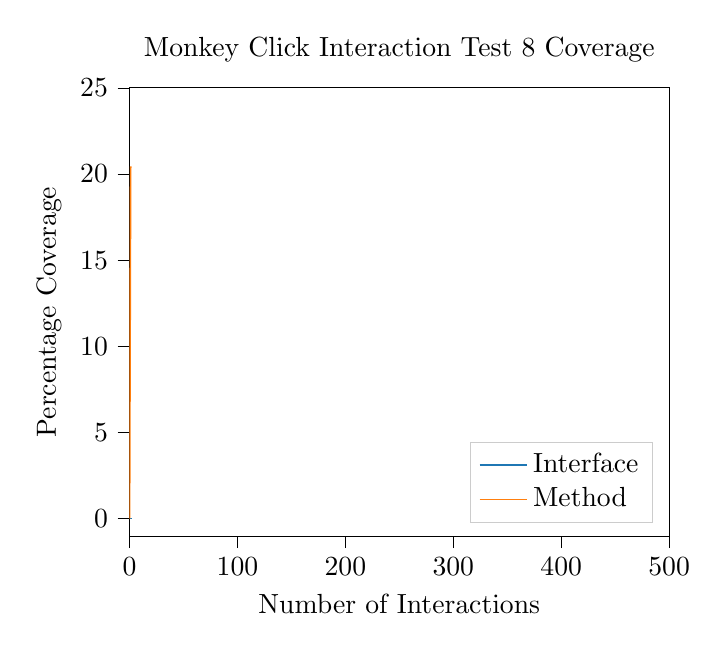
\begin{tikzpicture}

\definecolor{darkgray176}{RGB}{176,176,176}
\definecolor{darkorange25512714}{RGB}{255,127,14}
\definecolor{lightgray204}{RGB}{204,204,204}
\definecolor{steelblue31119180}{RGB}{31,119,180}

\begin{axis}[
legend cell align={left},
legend style={
  fill opacity=0.8,
  draw opacity=1,
  text opacity=1,
  at={(0.97,0.03)},
  anchor=south east,
  draw=lightgray204
},
tick align=outside,
tick pos=left,
title={Monkey Click Interaction Test 8 Coverage},
x grid style={darkgray176},
xlabel={Number of Interactions},
xmin=-0.1, xmax=500,
xtick style={color=black},
y grid style={darkgray176},
ylabel={Percentage Coverage},
ymin=-1.02, ymax=25,
ytick style={color=black}
]
\addplot [semithick, steelblue31119180]
table {%
0 0
1 0
2 0
};
\addlegendentry{Interface}
\addplot [semithick, darkorange25512714]
table {%
0 0
1 20.4
2 20.4
};
\addlegendentry{Method}
\end{axis}

\end{tikzpicture}
